\documentclass[../summary.tex]{subfiles}

\begin{document}
	
	\section{Climate}
		
		\subsection{Climate trends and causes}
			\subsubsection{Climate change over geological cycles}
				We know climate change is partly a natural phenomenon because of the research done with Antarctic ice. Figure \ref{fig:1-antarctic-ice-records} clearly shows a natural cycle in temperatures over the last 800,000 years. Other evidence pointing to this conclusion can be found in landscapes which have been altered by moving glacial ice.
				\begin{figure}[h]
					\centering
					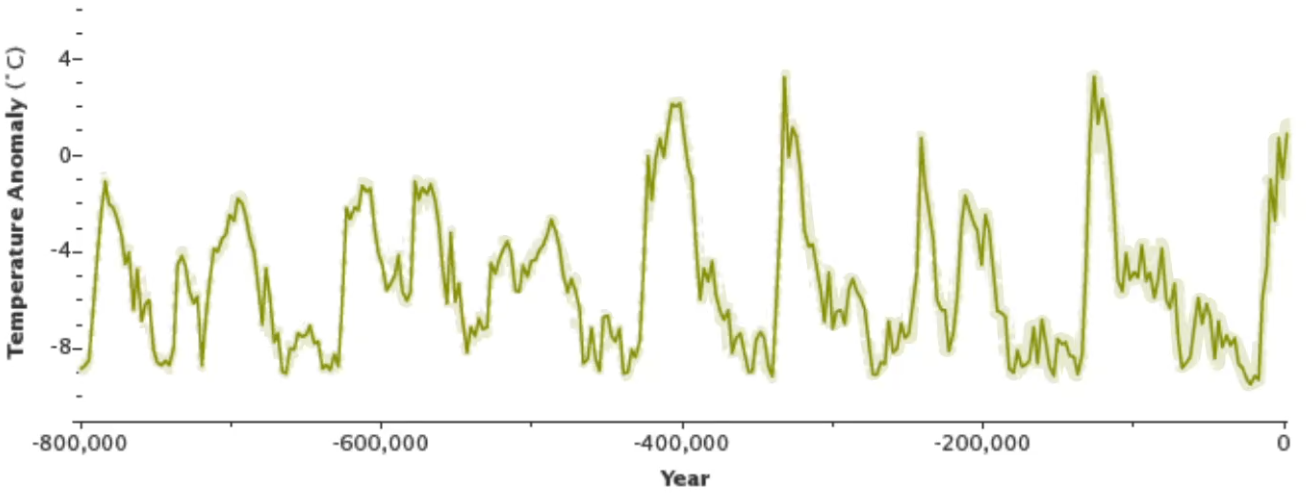
\includegraphics[width=0.7\linewidth]{../images/1-antarctic-ice-records.png}
					\caption{Antarctic ice records}
					\label{fig:1-antarctic-ice-records}
				\end{figure}
			
			\subsubsection{Causes of climate change}
				There are a few factors which cause the change in climate on earth:
				\begin{itemize}
					\item Variations in the earth's orbit around the sun (eccentricity)
					\item The axis of the Earth from pole to pole is tilted compared to this plane of movements, this is time dependent (obliquity)
					\item Precession of the Earth. 
				\end{itemize}
				Of these especially obliquity is important. It can lead to very hot summers and very cold winters without a lot of snowfall. This leads to a shrinkage in the ice coverage of the Earth which leads to ever warmer temperatures. This feedback loop amplifies itself (albedo feedback). Another factor is the physical place of land mass. If it is close to the poles, ice can easily form and reflect heat back into space. Volcanic explosions are known to have an influence as well due to their tendency to throw light blocking particles in the atmosphere. Lastly the activity of the sun itself plays a role in the climate of the earth. \\
				\\
				Us humans have had an impact since the industrial revolution by throwing tiny particles in the air due to burning fossil fuels, cooling the earth. This effect is overshadowed by the fact that we emit a lot of greenhouse gasses whilst we burn the same fossil fuels. 
		\subsection{Climate targets and pathways}
		
		\subsection{Climate mitigation}
		
		\subsection{What can we expect for the future}
	
\end{document}